\documentclass{article}

% Packages
\usepackage[utf8]{inputenc}

\usepackage{amsmath, bm}
\usepackage{graphicx}
\usepackage{amssymb}
\usepackage{float}
\usepackage{caption}
\usepackage{subcaption}

\title{3A3 Compressor Lab Report}
\author{[Louis Pender]}
\date{\today}

\begin{document}

\maketitle

\section{Abstract}
% Provide a brief summary of the lab report, including the objective, methodology, and key findings.

\section{Introduction}

Two compressor setups were used in this experiment.
One with pure water, where the speed could be varied, and another using glycerine, a more viscous solution of 60\%
glycerine and 40\% water, where the compressor speed was fixed.
For the water setup, the flow rates were varied by screw valves at the inlet and outlet which were measured by pressure difference of a venturi flume.
The glycerine setup the flow rate was varied by a screw valve at outlet of the compressor, and was measured by timing a fixed volume of fluid.

\section{Theory}
% Describe the experimental setup, equipment used, and the steps followed during the experiment.

% Sketch the compressor rotor marking the inlet and exit flow directions and indicate which side
% of the blade is the suction surface and has the lowest average pressure and which is the pressure
% surface with the highest average pressure. Explain how you can determine which side is which.

% Sketch done on paper



\subsection{Non Dimensional Groups}

% Define a suitable non-dimensional cavitation number. Plot a graph of non-dimensional
% cavitation number against non-dimensional flow coefficient.


The reynolds number takes a standard form of:
\begin{equation}
    Re = \frac{\rho UD}{\mu} = O\left( \frac{\rho ND^2}{\mu} \right)
\end{equation}
The factor of a half the diameter for outer blade velocity is omitted to simplify the non dimensionalisation. 

Two more non-dimensional groups are often used to characterise the flow in a compressor, the flow coefficient and the pressure rise coefficient.
These are defined as follows:
\begin{align}
    \text{Flow Coefficient} &= \frac{\dot{Q}}{ND^3} \\
    \text{Pressure Coefficient} &= \frac{\Delta p}{\rho N^2 D^2}
\end{align}

Cavitation is caused by local pressure drops below that of the vapour pressure of the fluid, causing the fluid to vaporise.
The collapse of these bubbles can cause high pressure waves and damage to the impeller.
It is therefore important to predict the conditions under which cavitation is likely to occur.

It would also be expected that the further the local pressure drops below the vapour pressure, the more likely cavitation is to occur.
A non-dimensional number that could be used to predict cavitation would be the difference between the local pressure and the vapour pressure, divided by the dynamic pressure, given below.
\begin{equation}
    C_t = \frac{p - p_v}{\frac{1}{2}\rho v^2}
\end{equation}
At the inlet, where the pressure is predicted to be the lowest, $v = N \frac{D_1}{2}$
This gives a non-dimensional cavitation number of:
\begin{equation}
    C_t = 8\frac{p - p_v}{\rho (ND_1)^2}
\end{equation}
Cavitation was predicted to occur at the inlet of the compressor, where the velocity is highest and so pressure lowest.

To obtain the cavitation number $C_t$ at the inlet of the compressor, the pressure at the inlet of the compressor is required.
This was obtained by working backwards from the pressure at the discharge point being atmospheric.
The height of the reservoir discharge and outlet of the compressor is given as 570mm. The pressure loss from the
venturi flume is negligible and for the cases where the inlet valve was adjusted, there is no pressure drop through the fully open exit valve.
The pressure at the inlet of the compressor is therefore given by:
\begin{equation}
    p_1 =  P_a + \rho g h - \Delta p
\end{equation}


\subsection{Flow measurements}

For the water setup, the flow rate was measured using a venturi flume, which measures the pressure difference across a constriction in the flow.
\begin{equation}
    \dot{m} = C_f A_1 \sqrt{\frac{2\rho_w \Delta p}{1 - \left( \frac{A_1}{A_2} \right)^2}}
\end{equation}
The calibrated discharge coefficient, and geomtry of the venturi flume were given in the form of a constant $a=0.193$ such that $\dot{m}=a \sqrt{\Delta p}$

For the glycerine setup, the flow rate was measured by timing a fixed volume of 15L of the solution.
The flow rate was therefore given by:
\begin{equation}
    \dot{Q} = \frac{V}{T}
\end{equation}
Which can easily be converted to mass flow rate using the known density $\rho_g$ of the glycerine solution.

% Velocity triangle on paper

% Using the mass flow rate and the impeller measurements, determine the radial velocity at the
% inlet to the blade at maximum flow condition, this is the starting value when valves are fully
% open. Non-dimensionalise your value by the blade speed.
Assuming incompressibility, the inlet and outlet radial component of velocity can simply be calculated from continuity.
\begin{equation}
    \dot{Q} = 2\pi r_1 v_1 = 2\pi r_2 v_{2r}
\end{equation}

For the water setup at maximum flow condition, both inlet and outlet valves are fully open.
Then, rearanging for the radial velocity at the inlet gives $V_1 = 1.74 m/s$.

This can be non-dimensionalised by the inlet blade speed to give:
\begin{equation}
    \frac{V_1}{U_1} = \frac{2\dot{Q}}{\pi N D_1 D_2 h}
\end{equation}

% Draw a velocity triangle for this situation and determine the relative velocity at the inlet to the
% rotor blade. 

\begin{figure}[H]
    \centering
    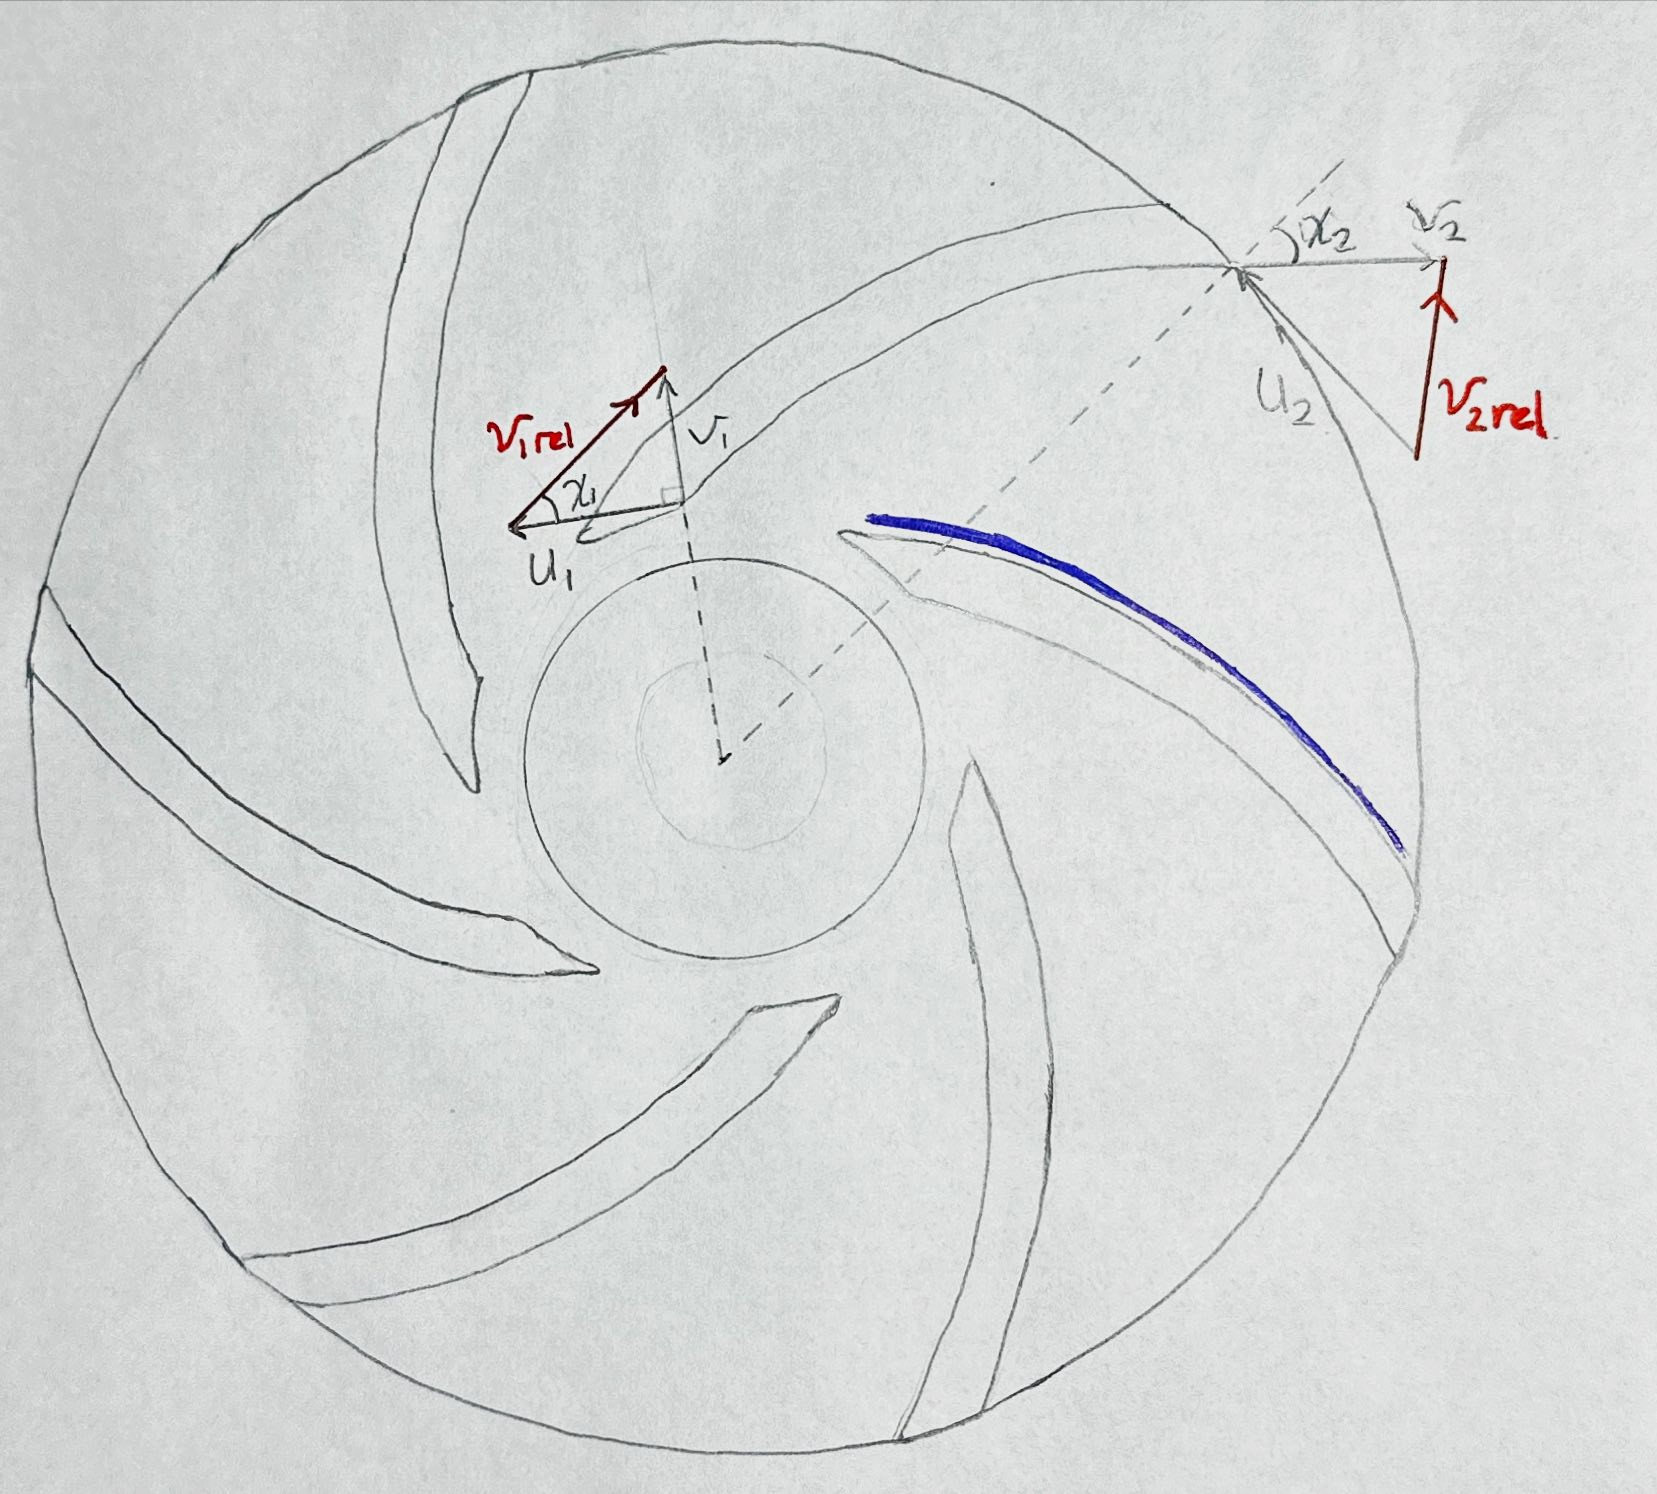
\includegraphics[width=0.6\textwidth]{velocity_diagrams.jpg}
    \caption{Compressor sketch and velocity diagrams. The high pressure surface is indicated by the blue line, with the suction surface on the opposite side of the channel.}
    \label{fig:vel_diagrams}
\end{figure}

% Use this velocity, the inlet diameter of the impeller and the kinematic viscosity of
% water to estimate the Reynolds number for the compressor. The magnitude of this Reynolds
% number will be comparable to values that you are familiar with for pipe flow



\subsection{Viscosity measurements}
% viscosity theory.

The viscosity of water is well known at standard conditions, however the viscosity of the glycerine solution is not.
However, using thin film theory, the time taken for a fluid to travel a specific distance can be used to determine the viscosity of the fluid.

\begin{equation}
    \mu \propto \frac{T\rho}{L}
\end{equation}
    
Where $\mu$ is the dynamic viscosity, $T$ is the time taken for the fluid to travel a distance $L$, and $\rho$ is the density of the fluid.
This can be used to determine the ratio of dynamic viscosities
\section{Results}
% Present the data obtained from the experiment, including tables, graphs, and figures.

% Plot all the five measured pressure rise characteristics on a single graph. Ensure the graph is
% sufficiently large and has a true zero on both axes. The 5 curves are: 2x full speed and 2x half
% speed for the water circuit and 1x full speed for the glycerine circuit.

\subsection{Impeller Geometry}

\begin{figure}[H]
    \centering
    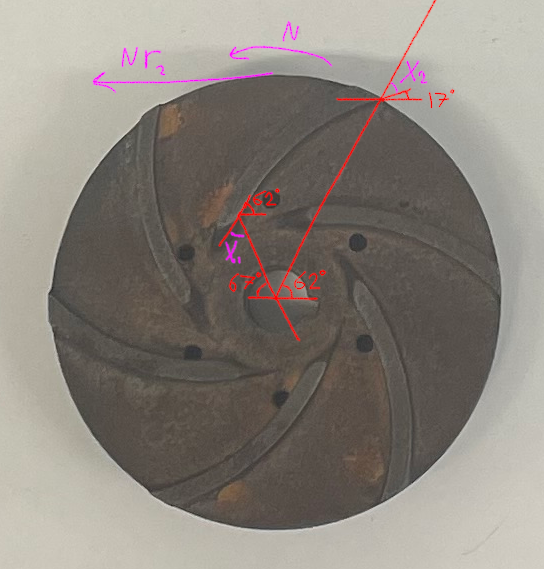
\includegraphics[width=0.6\textwidth]{impeller_annotations.png}
    \caption{Example image}
    \label{fig:impeller_annotations}
\end{figure}

And so angles of impeller blades to the radial direction are given by:
\begin{alignat}{2}
    \chi_1 &= 180 - 62 - 67 &= 51^\circ \notag \\
    \chi_2 &= 62 - 17 &= 45^\circ \notag
\end{alignat}

These values are shown in the table below, along with additional inlet and outlet diameter measurements with callipers.

\begin{table}[H]
    \centering
    \begin{tabular}{|c|c|}
        \hline
        \textbf{Quantity} & \textbf{Value} \\
        \hline
        Inlet Diameter $D_1$ & 25.2 mm \\
        Outlet Diameter $D_2$ & 79.3 mm \\
        Blade Span $h$ & 6.40 mm \\
        Blade Width $b$ & 3.9 mm \\
        Inlet Blade Angle $\chi_1$ & $51^\circ$ \\
        Outlet Blade Angle $\chi_2$ & $45^\circ$ \\
        \hline
    \end{tabular}
    \caption{Impeller geometry measurements.}
    \label{tab:impeller_geometry}
\end{table}

The ambient pressure was measured as $754$ mmHg, corresponding to $100.56$ kPa.

\subsection{Viscosiy measurements}

At the ambient conditions the density of water is $998.2 kg/m^3$.
The density of the glycerine solution was known to be $1170 kg/m^3$.

\begin{table}[H]
    \centering
    \begin{tabular}{|c|c|c|}
        \hline
        \textbf{Length} $(m)$ & \textbf{Time} (s) & \textbf{Density} ($kg/m^3$) \\
        \hline
        10 & 40.35 & 998.2 \\
        2 & 102.01 & 1170 \\
        \hline
    \end{tabular}
    \caption{Time taken for 10mL of fluid to travel a specific length at $18.3^\circ C.$}
    \label{tab:viscosity}
\end{table}

The ratio of dynamic viscosities of the fluids is given by the ratio of time to length.

\subsection{Compressor Data}

\begin{figure}[H]
    \centering
    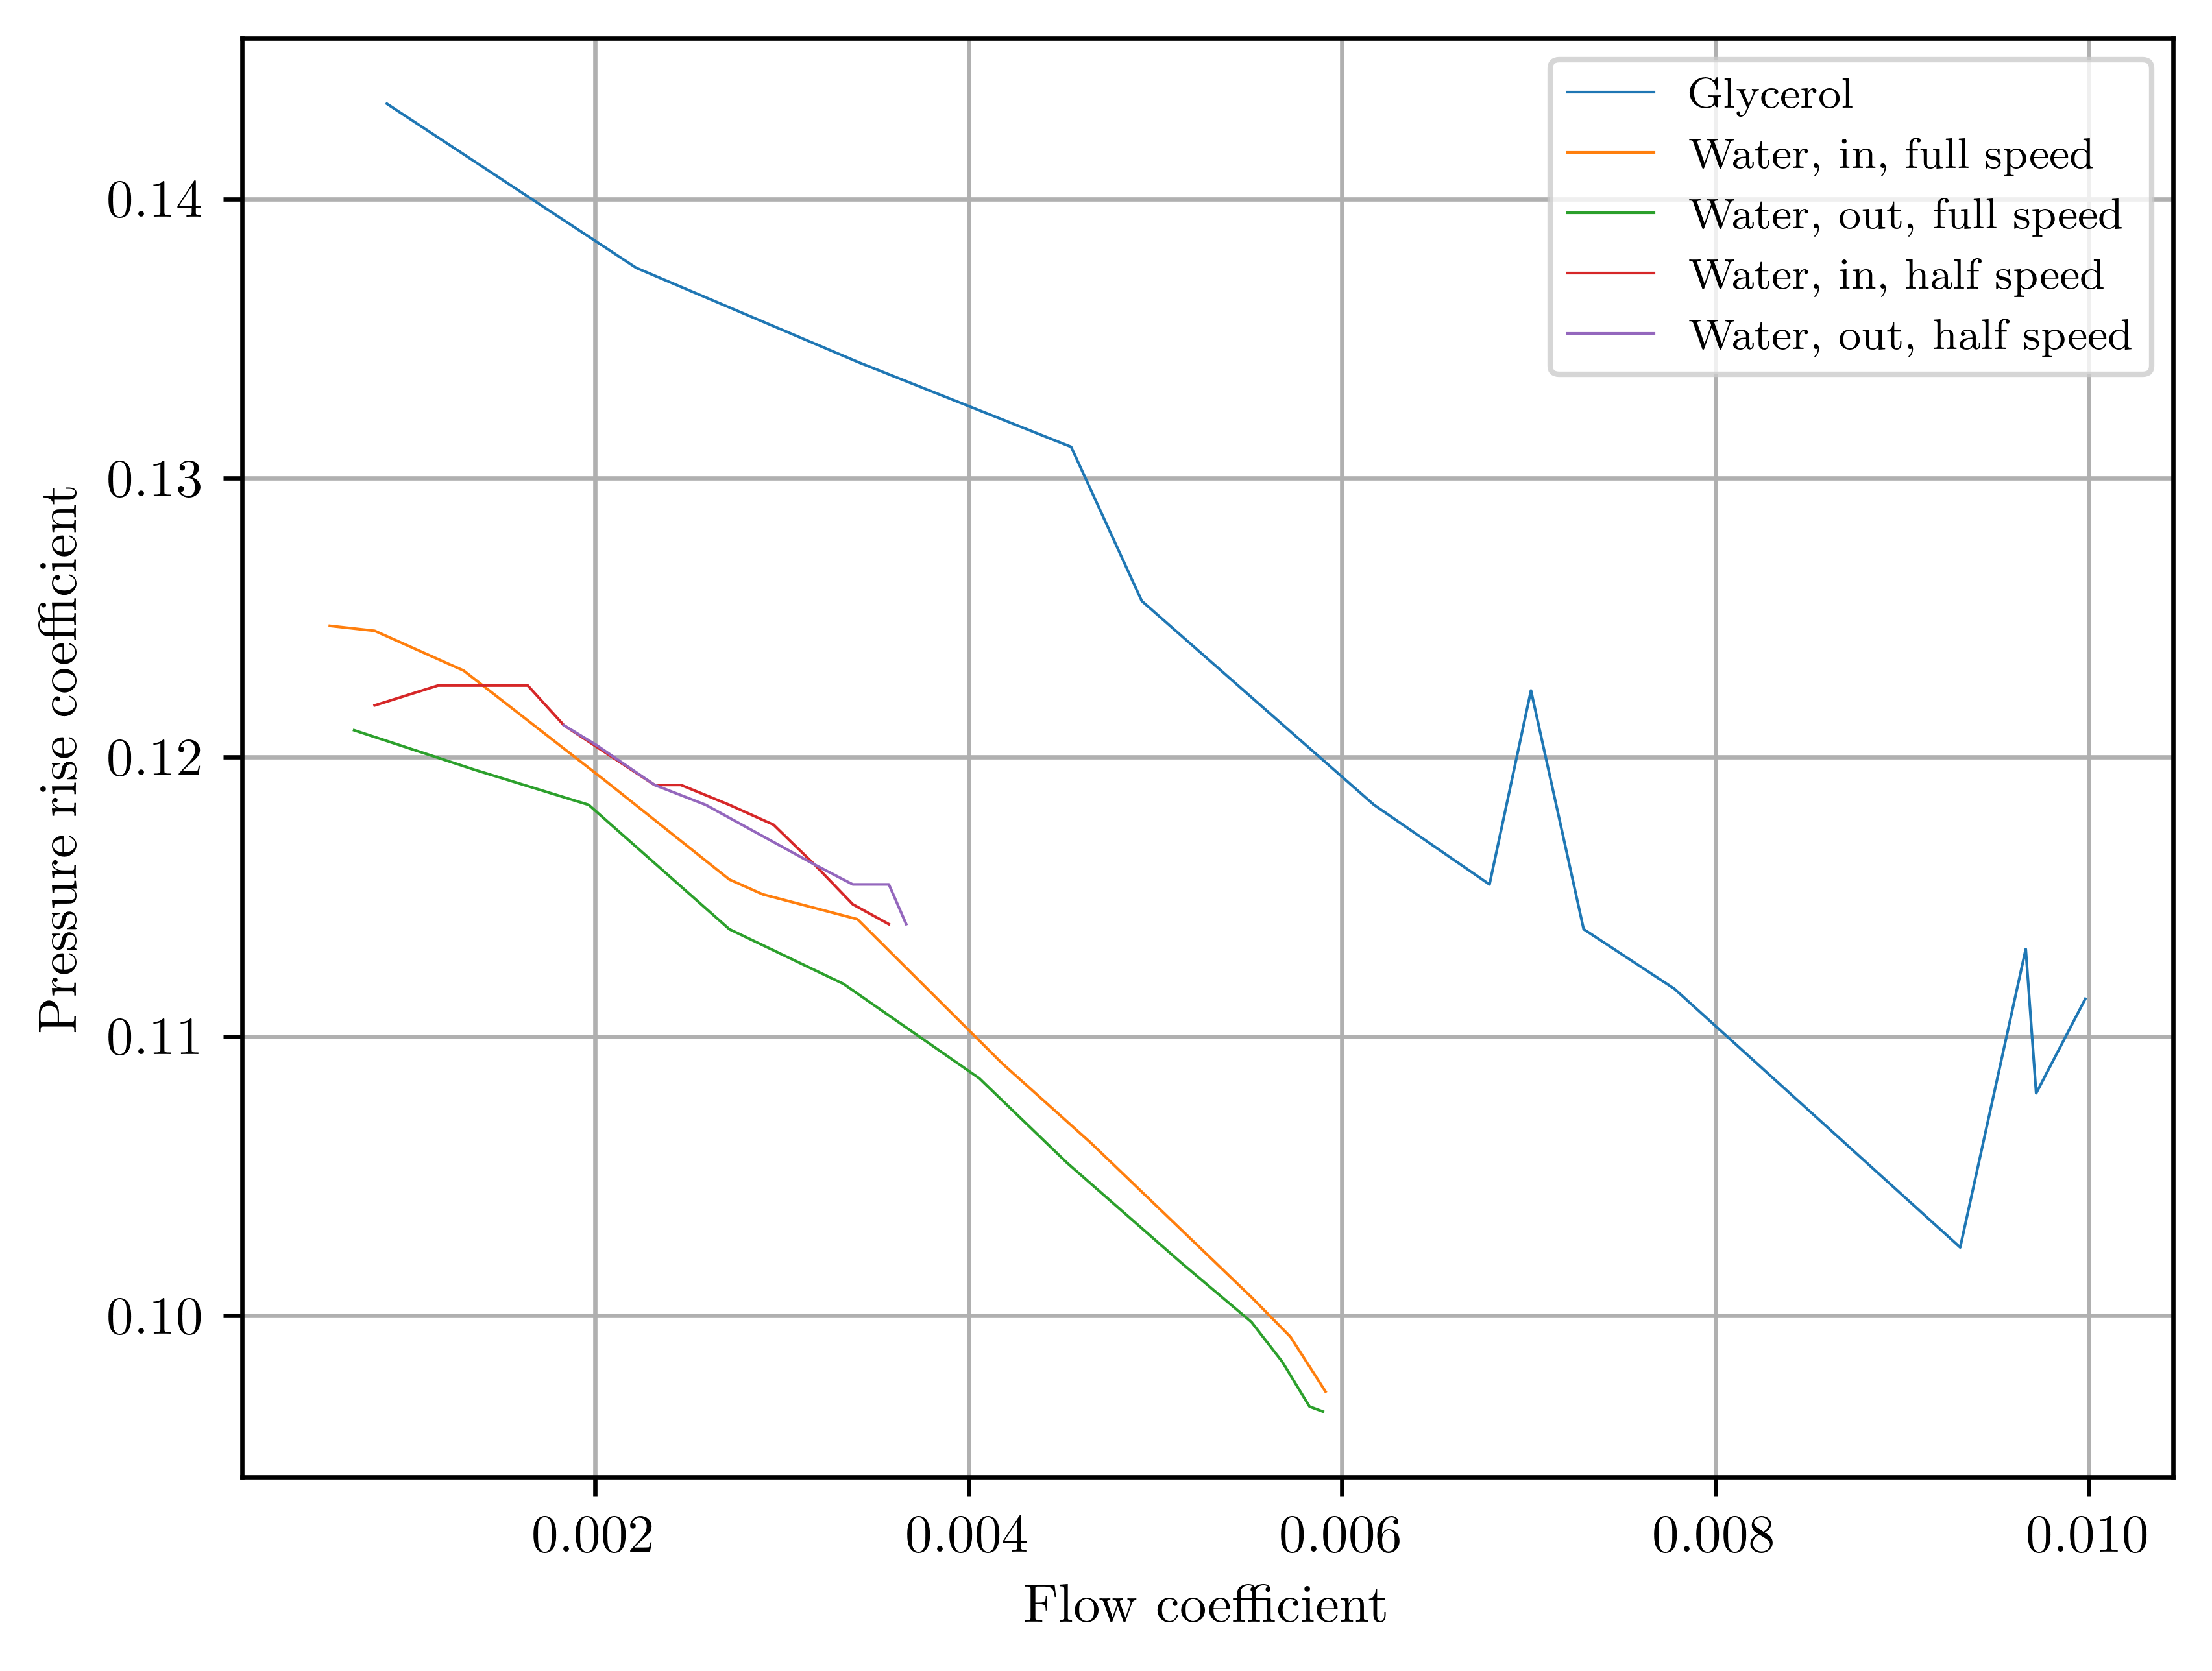
\includegraphics[width=0.99\textwidth]{compressor_non_dims.png}
    \caption{Non-dimensional pressure rise coefficient against non-dimensional flow coefficient various compressors conditions and setups.}
    \label{fig:compressor_non_dims}
\end{figure}

% Pressure Rise Coefficient against Tip Reynolds number.

\section{Discussion}
% Analyze and interpret the results, discussing their significance and any observations or trends.

For all compressor arrangements, the pressure coefficient decreases with increasing flow coefficient.


% Explain why throttling the water compressor at inlet and exit produce different cavitation
% results. Also explain why the pressure rise is similar when cavitation is not present.

why is pressure rise similar to when caviation is not present?

% Do the results agree with what you expect for:
%% Change of pressure rise with flow rate

The pressure coefficients for water at lower compressor speeds are higher than those at higher speeds, as expected.


%% Change of pressure rise with Reynolds number. Reference to figure 3 may be useful -
%% k/d is comparable to the roughness height of the blade surface divided by the channel span

%% Change in cavitation with rotor speed and throttle location? Sketch two velocity
%% triangles, one at a nominal design condition and when the flow coefficient is much lower.

Cavitation bubbles were observed to coalesce to form larger bubbles, which then collapsed.

%$ Can you explain the differences? Note that the two compressors do not give exactly the same
%% pressure rise-flow rate characteristics, and so care must be taken in comparing the effect of
%% Reynolds number.


% Suggest a reason why the venturi might not be suitable for measuring the flow rate of the
% glycerine solution.
The venturi flume 

\section{Conclusion}
% Summarize the main findings of the experiment and draw conclusions based on the results.

\end{document}
